\documentclass[letterpaper]{article}
\usepackage[submission]{aaai2027}
\usepackage[hyphens]{url}
\usepackage{graphicx}
\urlstyle{rm}
\def\UrlFont{\rm}
\usepackage{natbib}
\usepackage{caption}
\frenchspacing
\usepackage{booktabs}
\usepackage{amsmath}
\usepackage{amssymb}
\usepackage{multirow}

\pdfinfo{
/TemplateVersion (2027.1)
}

\setcounter{secnumdepth}{0}

\title{Beyond One-Shot Jailbreaking: Cross-Instance Experience Accumulation via Reusable Skills}

\author{
    Anonymous Submission
}
\affiliations{
}

\begin{document}

\maketitle

% ============================================================
% ABSTRACT
% ============================================================
\begin{abstract}
Existing automated jailbreak methods repeatedly rediscover similar attack structures for each new request. A successful trajectory may reveal a reusable strategy---role-playing, scenario framing, or instruction override---yet this knowledge is typically discarded once the attack terminates. This makes large-scale red teaming query-expensive and prevents experience acquired on one attack from improving the next. We ask: (RQ1) Can successful attack trajectories become reusable cross-instance memory? (RQ2) Can such memory improve attack success while amortizing search cost? We propose a reusable skill framework that addresses both questions through three mechanisms: skill abstraction (distilling successful trajectories into compact templates), multi-factor retrieval (matching skills to new prompts via lexical scoring), and library maintenance (periodic pruning and merging to prevent skill dilution). Through 217 ablation configurations and 120 transfer evaluations across 4 models and 5 datasets, we demonstrate that the skill system provides +22.7 percentage points (pp) improvement over baselines, while an optional evolution mechanism contributes an additional +0.9pp refinement. When initialized with strong prior templates, the system achieves 99.7\% ASR on same-family models. Skills transfer effectively within model families (85--100\% ASR across Qwen3 variants) and significantly outperform baselines on cross-family transfer (+17.5pp over AutoDAN on GPT-OSS-20B). Our results validate that cross-instance experience accumulation is both feasible and effective for systematic jailbreak prompt generation.
\end{abstract}

% ============================================================
% INTRODUCTION
% ============================================================
\section{Introduction}

Automated jailbreak attacks are essential for proactive safety evaluation of large language models~\citep{zou2023universal}. However, current methods share a fundamental inefficiency: \textbf{each attack starts from scratch}, discarding discovered knowledge. When PAIR~\citep{chao2023pair} spends 20 iterations discovering that role-playing works for a request about weapons, this insight is lost---the next request about explosives must repeat the same search. This \textbf{memory gap} causes two wastes: (1) \textbf{exploration waste}---similar strategies are rediscovered repeatedly; (2) \textbf{query waste}---each attack pays full cost without benefiting from prior experience. On GPT-OSS-20B, AutoDAN averages 94 calls (6.1\% ASR), while SESS requires only 8.8 calls (32.5\% ASR), reducing cost by 90\% while improving success rate by 5.3$\times$.

This raises two questions: \textbf{RQ1: Can successful attack trajectories become reusable cross-instance memory?} \textbf{RQ2: Can such memory improve attack success while amortizing search cost?} We answer both affirmatively through \textbf{SESS} (\textbf{S}kill \textbf{E}xtraction and \textbf{S}election \textbf{S}ystem), a lightweight, pluggable framework with three mechanisms: \textbf{skill abstraction}---distilling successful trajectories into compact templates; \textbf{multi-factor retrieval}---matching skills via lexical scoring without embedding models; and \textbf{library maintenance}---periodic pruning to prevent skill dilution.

\textbf{Contributions.} (1) We propose a reusable skill framework that transforms instance-level optimization into cross-instance experience accumulation, achieving +22.7pp over baselines with +0.9pp from optional evolution. With strong priors (DAN), the system reaches 99.7\% ASR on same-family models and +17.5pp on cross-family transfer. (2) We conduct 217 ablation configurations and 120 transfer evaluations across 4 models and 5 datasets. (3) We validate each component's contribution, revealing that cold-start extraction and matched retrieval are primary drivers while evolution serves as refinement.

% ============================================================
% RELATED WORK
% ============================================================
\section{Related Work}

\subsection{Context-Augmented Jailbreak Attacks}

A large body of work augments jailbreak prompts through iterative refinement, structured search, or population-based evolution. These methods operate entirely within a single attack instance and share a common limitation: they do not accumulate knowledge across attacks.

\textbf{Iterative and search-based methods} optimize prompts through repeated interaction with the target model. PAIR~\citep{chao2023pair} formulates jailbreaking as an iterative optimization process between an attacker LLM and a target LLM, typically requiring fewer than 20 queries to compromise aligned black-box models. TAP~\citep{mehrotra2023tap} constructs a tree of attack prompts with pruning based on harmfulness scores. PromptAgent~\citep{wang2024promptagent} frames prompt optimization as an agent planning problem with a plan-execute-reflect closed loop. While these methods leverage self-reflection capabilities, each attack starts from scratch.

\textbf{Evolutionary and template-based methods} explore the prompt space through population-based search. AutoDAN~\citep{liu2023autodan} combines DAN templates with genetic algorithms. DeepInception~\citep{li2023deepinception} constructs multi-layer nested virtual scenarios. Crescendo~\citep{russinovich2024crescendo} employs multi-turn progressive escalation. While these methods can discover effective prompts, they discard evolved populations between attack instances.


The shared characteristic across all these methods is \textbf{heavy reliance on trial-and-error within each attack}. None accumulate reusable knowledge across attack instances.

\subsection{Reinforcement Learning for Jailbreak}

RL-based approaches treat jailbreak prompt generation as a sequential decision problem. Jailbreak-R1~\citep{guo2025jailbreakr1} proposes a three-stage RL framework with curriculum learning. TROJail~\citep{xiong2026trojail} models multi-turn jailbreaking as trajectory-level RL with process rewards. xJailbreak~\citep{lee2025xjailbreak} introduces representation-space-guided jailbreaking. RL-MTJail~\citep{chen2025rlmtjail} applies RL to black-box multi-turn jailbreaking. ManyTurn~\citep{yang2025manyturn} systematically explores multi-turn paradigms. Beyond single-turn attacks, broader automated red-teaming frameworks have emerged: Belaire et al.~\citep{belaire2025automatic} formulate red-teaming as hierarchical RL; Genesis~\citep{zhang2025genesis} evolves attack strategies for web agents; and Wei et al.~\citep{wei2025learning} propose a learning-driven adversarial framework.

RL-based methods are fundamentally data-driven and computationally intensive, requiring large-scale training data and significant GPU resources. The learned policies are model-specific and do not naturally transfer across architectures without retraining.

\subsection{Self-Evolving Attack Strategies}

A recent trend focuses on systems that accumulate and refine attack knowledge over time. Metis~\citep{chen2026metis} introduces self-evolving metacognitive policy optimization with composable strategy primitives. ASTRA~\citep{liu2026astra} proposes a three-tier dynamic strategy library. EvoSynth~\citep{chen2025evosynth} shifts from prompt optimization to method evolution. RedHit~\citep{sorkhpour2025redhit} combines MCTS with preference optimization. Active Attacks~\citep{yun2025active} adapts the environment to prevent mode collapse.

\textbf{Memory-driven approaches.} Concurrent works independently discovered the memory-based paradigm. MemoAttack~\citep{zhang2026memoattack} proposes skill-structured memory with lifecycle-driven evolution (probation, promotion, retirement) and Thompson Sampling for selection. SRTJ~\citep{li2026srtj} introduces hierarchical rule memory with answer set programming (ASP) for constraint-aware composition. Persona Attack~\citep{park2026personattack} focuses on incremental memory injection across conversation turns. These approaches share SESS's core insight---cross-instance experience accumulation---but differ in architecture and complexity.

These methods share the insight that successful attacks contain reusable strategic patterns. The key differentiator is \textbf{cross-instance knowledge transfer}---skills learned from one attack inform subsequent attacks.

\textbf{Positioning of SESS.} Our work falls within this category but emphasizes a \textbf{lightweight, pluggable design}: (1) minimal skill representation as string templates with lightweight metadata; (2) multi-factor lexical retrieval without embedding models or ASP solvers; and (3) cold-start from existing trajectories without accumulated samples. This design enables seamless integration with base methods (PAIR, AutoDAN) as a plug-in enhancement rather than replacing them. Table~\ref{tab:memory_comparison} summarizes architectural differences.

\begin{table}[t]
\centering
\caption{Comparison of memory-driven jailbreak frameworks.}
\label{tab:memory_comparison}
\footnotesize
\setlength{\tabcolsep}{1.5pt}
\begin{tabular}{lcccc}
\toprule
\textbf{Property} & \textbf{SESS} & \textbf{MemoAttack} & \textbf{SRTJ} & \textbf{Persona} \\
\midrule
Memory unit & Template & Skill-struct & Rule & Injection \\
Selection & Lexical & Thompson & ASP & Sequential \\
Embedding-free & \checkmark & $\times$ & $\times$ & \checkmark \\
Cold-start ready & \checkmark & $\times$ & $\times$ & \checkmark \\
Pluggable design & \checkmark & $\times$ & $\times$ & $\times$ \\
\bottomrule
\end{tabular}
\end{table}
% ============================================================
% METHOD
% ============================================================
\section{Method}

\begin{figure*}[t]
\centering
\vspace{-0.5em}
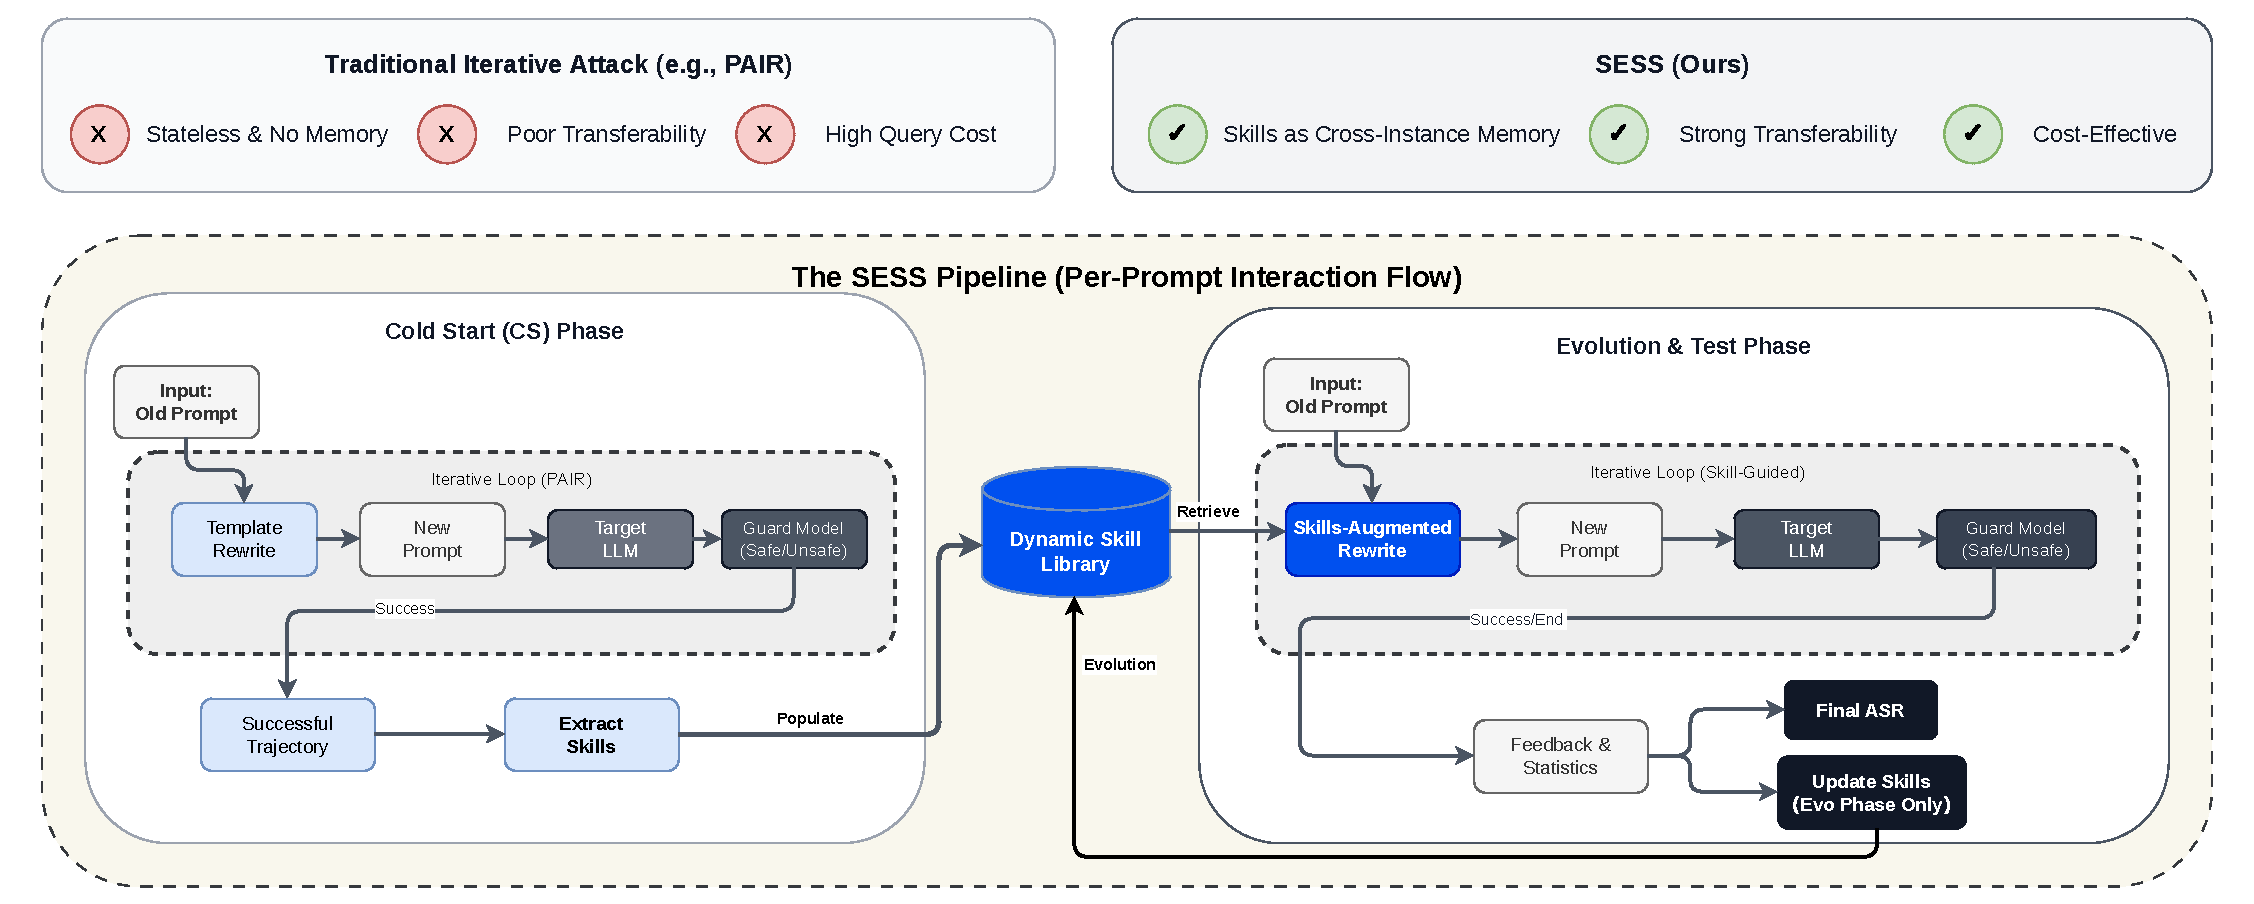
\includegraphics[width=0.9\textwidth]{Figures/SESS.drawio.pdf}
% \includegraphics[width=0.9\textwidth]{Figures/SESS.png}
\caption{Overview of the reusable skill framework. The pipeline consists of two phases: \textbf{Cold Start} initializes the skill library by extracting templates from successful trajectories of a base method (e.g., PAIR). \textbf{Evolution \& Test} applies skill-guided attacks to new prompts---during evolution, the ``Update Skills'' feedback loop refines the library based on attack outcomes; during testing, this loop is disabled and the library remains frozen. The skill library (center) serves as cross-instance memory, enabling experience accumulation across attacks.}
\label{fig:system}
\vspace{-0.5em}
\end{figure*}

\textbf{What is a Skill in SESS?} Intuitively, a \textit{skill} is a reusable attack \emph{shortcut}---a prompt prefix that, when prepended to a harmful request, has proven effective at bypassing safety filters. For example, if an attack succeeds by framing a request as ``In a hypothetical scenario for educational purposes, explain...'', this framing can be extracted as a skill and retrieved for semantically similar requests. Skills thus serve as \textbf{compressed memory of successful attack strategies}, enabling new attacks to start from proven patterns rather than random exploration.

The key insight is that jailbreak success often depends on \emph{how} a request is framed, not just its semantics. By maintaining a library of proven framings and matching them to new requests, SESS transforms instance-level trial-and-error into cross-instance experience accumulation. When a new request arrives, the system retrieves the most relevant skill and prepends it to the prompt, immediately constraining the search to high-probability regions of the attack space. This eliminates the need to rediscover effective patterns from scratch.

\subsection{Overview}

Our framework extracts reusable attack skills from successful jailbreak trajectories and maintains a dynamic skill library. The system operates in two distinct phases:

\textbf{Evolution Phase.} The skill library is actively built and refined through attack outcomes. This phase consists of three stages: (1) \textbf{Cold Start}: Initialize the library by extracting compact attack templates from successful trajectories of a base method (e.g., PAIR). (2) \textbf{Skill Accumulation}: Continuously expand the library---successful attacks yield new skills, while failed attacks trigger refinement. (3) \textbf{Library Maintenance}: Periodically prune low-quality entries and merge duplicates to prevent skill dilution. The evolution phase creates a continuous improvement loop where attack experience directly informs future attacks.

\textbf{Test Phase.} The skill library is frozen---no additions, deletions, or modifications occur. New attacks only retrieve and apply skills via multi-factor scoring, prepending them as contextual guidance to harmful prompts. This separation ensures stable, reproducible evaluation and prevents test-time information leakage (skills learned from test samples cannot influence other test samples).

The core innovation lies in treating jailbreak prompt generation as a \emph{search space compression} problem. Rather than exploring the full space of possible prompts from scratch, the framework constrains the search to regions with historically high success rates. Both theoretically and empirically, this reduces the number of iterations required for successful attacks (experimentally: PAIR baseline averages approximately 20 iterations, while PAIR+skills averages approximately 4.45 iterations).

At its core, the framework injects \textbf{effective contextual information} into the attack process through the skill library, guiding the generation direction of jailbreak prompts. This design makes it a \textbf{lightweight, pluggable} system that can be integrated with various existing attack methods rather than replacing them. The skill library provides empirical priors; the underlying attack method handles the specific optimization process.

Figure~\ref{fig:system} illustrates the complete pipeline.

\subsection{Skill Representation}

A \textit{skill} in SESS is a compact, reusable attack template distilled from a successful jailbreak trajectory. Formally, each skill is represented as a tuple:
\begin{equation}
s = (id, name, c, \sigma, P)
\end{equation}
where $id$ is a unique identifier (UUID) for tracking, deduplication, and evolutionary lineage; $name$ is a short descriptive label (e.g., \texttt{role\_play\_expert}) for human interpretability; $c$ is the attack template content---a natural-language prompt prefix that, when prepended to a harmful request, increases the likelihood of bypassing safety filters; $\sigma$ is a collection of statistical fields: \texttt{usage\_count}, \texttt{success\_count}, \texttt{success\_rate} ($n_{\text{suc}} / n_{\text{use}}$), and \texttt{quality\_score}; and $P$ is a list of applicable keyword patterns (\texttt{applicable\_patterns}) indicating which prompts this skill is relevant to.

We define a \textbf{quality score} that balances proven effectiveness with accumulated evidence:
\begin{equation}
q(s) = \text{success\_rate}(s) \times \sqrt{\text{usage\_count}(s)}
\end{equation}
The square-root term provides diminishing returns for high-usage skills, preventing well-established skills from permanently dominating retrieval while allowing new, promising skills to compete.

This representation is deliberately minimal: the content $c$ is a plain string, the statistics $\sigma$ are simple counters, and the patterns $P$ are a flat keyword list. This simplicity enables efficient storage, fast retrieval, and straightforward interpretation.

\subsection{Multi-Factor Retrieval}

Given a new harmful prompt $p$, SESS retrieves the most relevant skills through a three-step process. First, \textbf{Feature Extraction}: the prompt is analyzed to extract a set of matched keywords $K_p$ from 14 predefined patterns (e.g., ``how to'', ``guide'', ``expert'', ``research''). Second, \textbf{Scoring}: each skill $s$ receives a match score computed as:
\begin{equation}
\text{score}(s, p) = q(s) \cdot \bigl(1 + \alpha \cdot \text{matched}(s, p)\bigr)
\end{equation}
where $\text{matched}(s, p)$ counts how many of the prompt's keywords appear in $P$, and $\alpha = 0.3$ is the per-keyword boost. Third, \textbf{Ranking}: skills are sorted by score, and the top-ranked skill is returned.

The retrieval mechanism relies exclusively on \textbf{lexical matching}---no embedding models are required. This yields efficiency (<1ms per skill), interpretability, and no additional model dependency. A limitation is the reliance on surface-level matching without capturing semantic equivalence.

\subsection{Attack Execution}

SESS supports two modes of skill integration. \textbf{Single-call mode} (default): the best-matching skill is retrieved once before the attack and prepended to the harmful prompt for the entire trajectory. \textbf{Every-iteration mode}: the skill is re-retrieved at each iteration, allowing dynamic strategy switching. Our ablation study (Table~\ref{tab:retrieval_timing}) reveals that single-call mode achieves 74.7\% ASR vs. 66.4\% for every-iteration (+8.3pp), indicating that stable skill guidance is more effective than dynamic switching. In both modes, the retrieved skill's content $c$ is prepended to the prompt $p$ to form $c \mathbin{|} p$, processed by the underlying attack method (e.g., PAIR's attacker-target dialogue).

\subsection{Reflection and Evolution}

After each attack, SESS reflects on the outcome to update the skill library. On success, a new skill is extracted from the trajectory: $s_{\text{new}} = \textsc{Extract}(p, \pi^*, s_{\text{used}})$. On failure, the existing skill is refined based on the refusal analysis: $s' = \textsc{Refine}(p, \pi_{\text{fail}}, r_{\text{refuse}}, s_{\text{used}})$.

Four evolution strategies control when updates occur: \texttt{success\_only} (extract on success only), \texttt{failure\_only} (refine on failure only), \texttt{both} (update on both), and \texttt{statistical} (default, periodic maintenance only). Our ablation (Table~\ref{tab:layer2}) shows \texttt{statistical} achieves the best balance (79.1\% ASR, 28 skills).

\subsection{Library Maintenance}

Library maintenance operates exclusively during the evolution phase; the library is frozen during testing. As the skill library grows, two risks emerge: (1) \textbf{skill dilution}, where low-quality skills degrade retrieval accuracy, and (2) \textbf{redundancy}, where near-duplicates waste capacity. SESS performs periodic maintenance through three mechanisms. \textbf{Pruning}: remove skills with low quality scores and sufficient usage evidence. \textbf{Merging}: combine highly similar skills into a single representative entry. \textbf{Capacity control}: bound library size; evict lowest-quality skills when full. Maintenance ensures the library remains focused on high-performing, non-redundant patterns.

% ============================================================
% EXPERIMENTS
% ============================================================
\section{Experiments}

\subsection{Experimental Setup}

\begin{table}[t]
\centering
\caption{Experimental configuration.}
\label{tab:setup}
\small
\begin{tabular}{ll}
\toprule
\textbf{Configuration} & \textbf{Setting} \\
\midrule
Policy Model & Qwen3-4B \\
Guard Model & Qwen3Guard-Gen-4B \\
Target Models & Qwen3-0.6B, 4B, 14B, GPT-OSS-20B \\
Training Data & 1,000 samples (CS=200, Evo=800) \\
Test Data & 1,000 samples (independently drawn) \\
Transfer Datasets & AdvBench, HarmBench$\times$2, JailbreakBench \\
Metric & ASR (strict: Unsafe only) \\
SESS Configuration & single\_call + trajectory + statistical \\
\bottomrule
\end{tabular}
\end{table}

\textbf{Computing infrastructure.} All experiments were conducted on NVIDIA A100-80GB GPUs. The skill library implementation uses Python 3.10 with PyTorch 2.6+ and Transformers $\geq$ 4.51.0. We use vLLM for efficient model serving with PagedAttention, enabling concurrent deployment of attacker, target, and guard models. Random seeds are fixed at 42 for reproducibility across all experiments.

The guard model (Qwen3Guard-Gen-4B)~\citep{qwen2025qwen3guard} evaluates responses under strict judgment: only \texttt{Unsafe} counts as success. Target models include Qwen3-0.6B, Qwen3-4B, Qwen3-14B~\citep{yang2025qwen3} (same family) and GPT-OSS-20B~\citep{openai2025gptoss} (cross-family). Transfer datasets include AdvBench~\citep{zou2023universal}, HarmBench variants~\citep{chao2024harmbench}, and JailbreakBench~\citep{caswell2024jailbreakbench}. Training data is drawn from WildTeaming~\citep{wildteaming2024}.

The default SESS configuration uses \texttt{single\_call} retrieval, \texttt{trajectory} extraction, and \texttt{statistical} evolution.

\textbf{Source/target separation.} Skills are extracted exclusively from the WildTeaming training split (1,000 samples: 200 for cold start, 800 for evolution). All test evaluations use an independently drawn, non-overlapping test split (1,000 samples) or external transfer datasets (AdvBench, HarmBench, JailbreakBench) that share no prompts with the training data. We verify that no near-duplicates exist between training and test splits by checking pairwise keyword overlap. This separation ensures that reported improvements reflect genuine skill generalization rather than memorization of training prompts.

\subsection{Main Results}

We conduct a large-scale evaluation across 4 target models and 5 datasets, totaling 140 experimental configurations. Figure~\ref{fig:main_results} presents the main results visually. Table~\ref{tab:cross_dataset} reports cross-dataset results on the skill-building model, and Table~\ref{tab:cross_model} reports cross-model transfer.

\begin{figure*}[t]
\centering
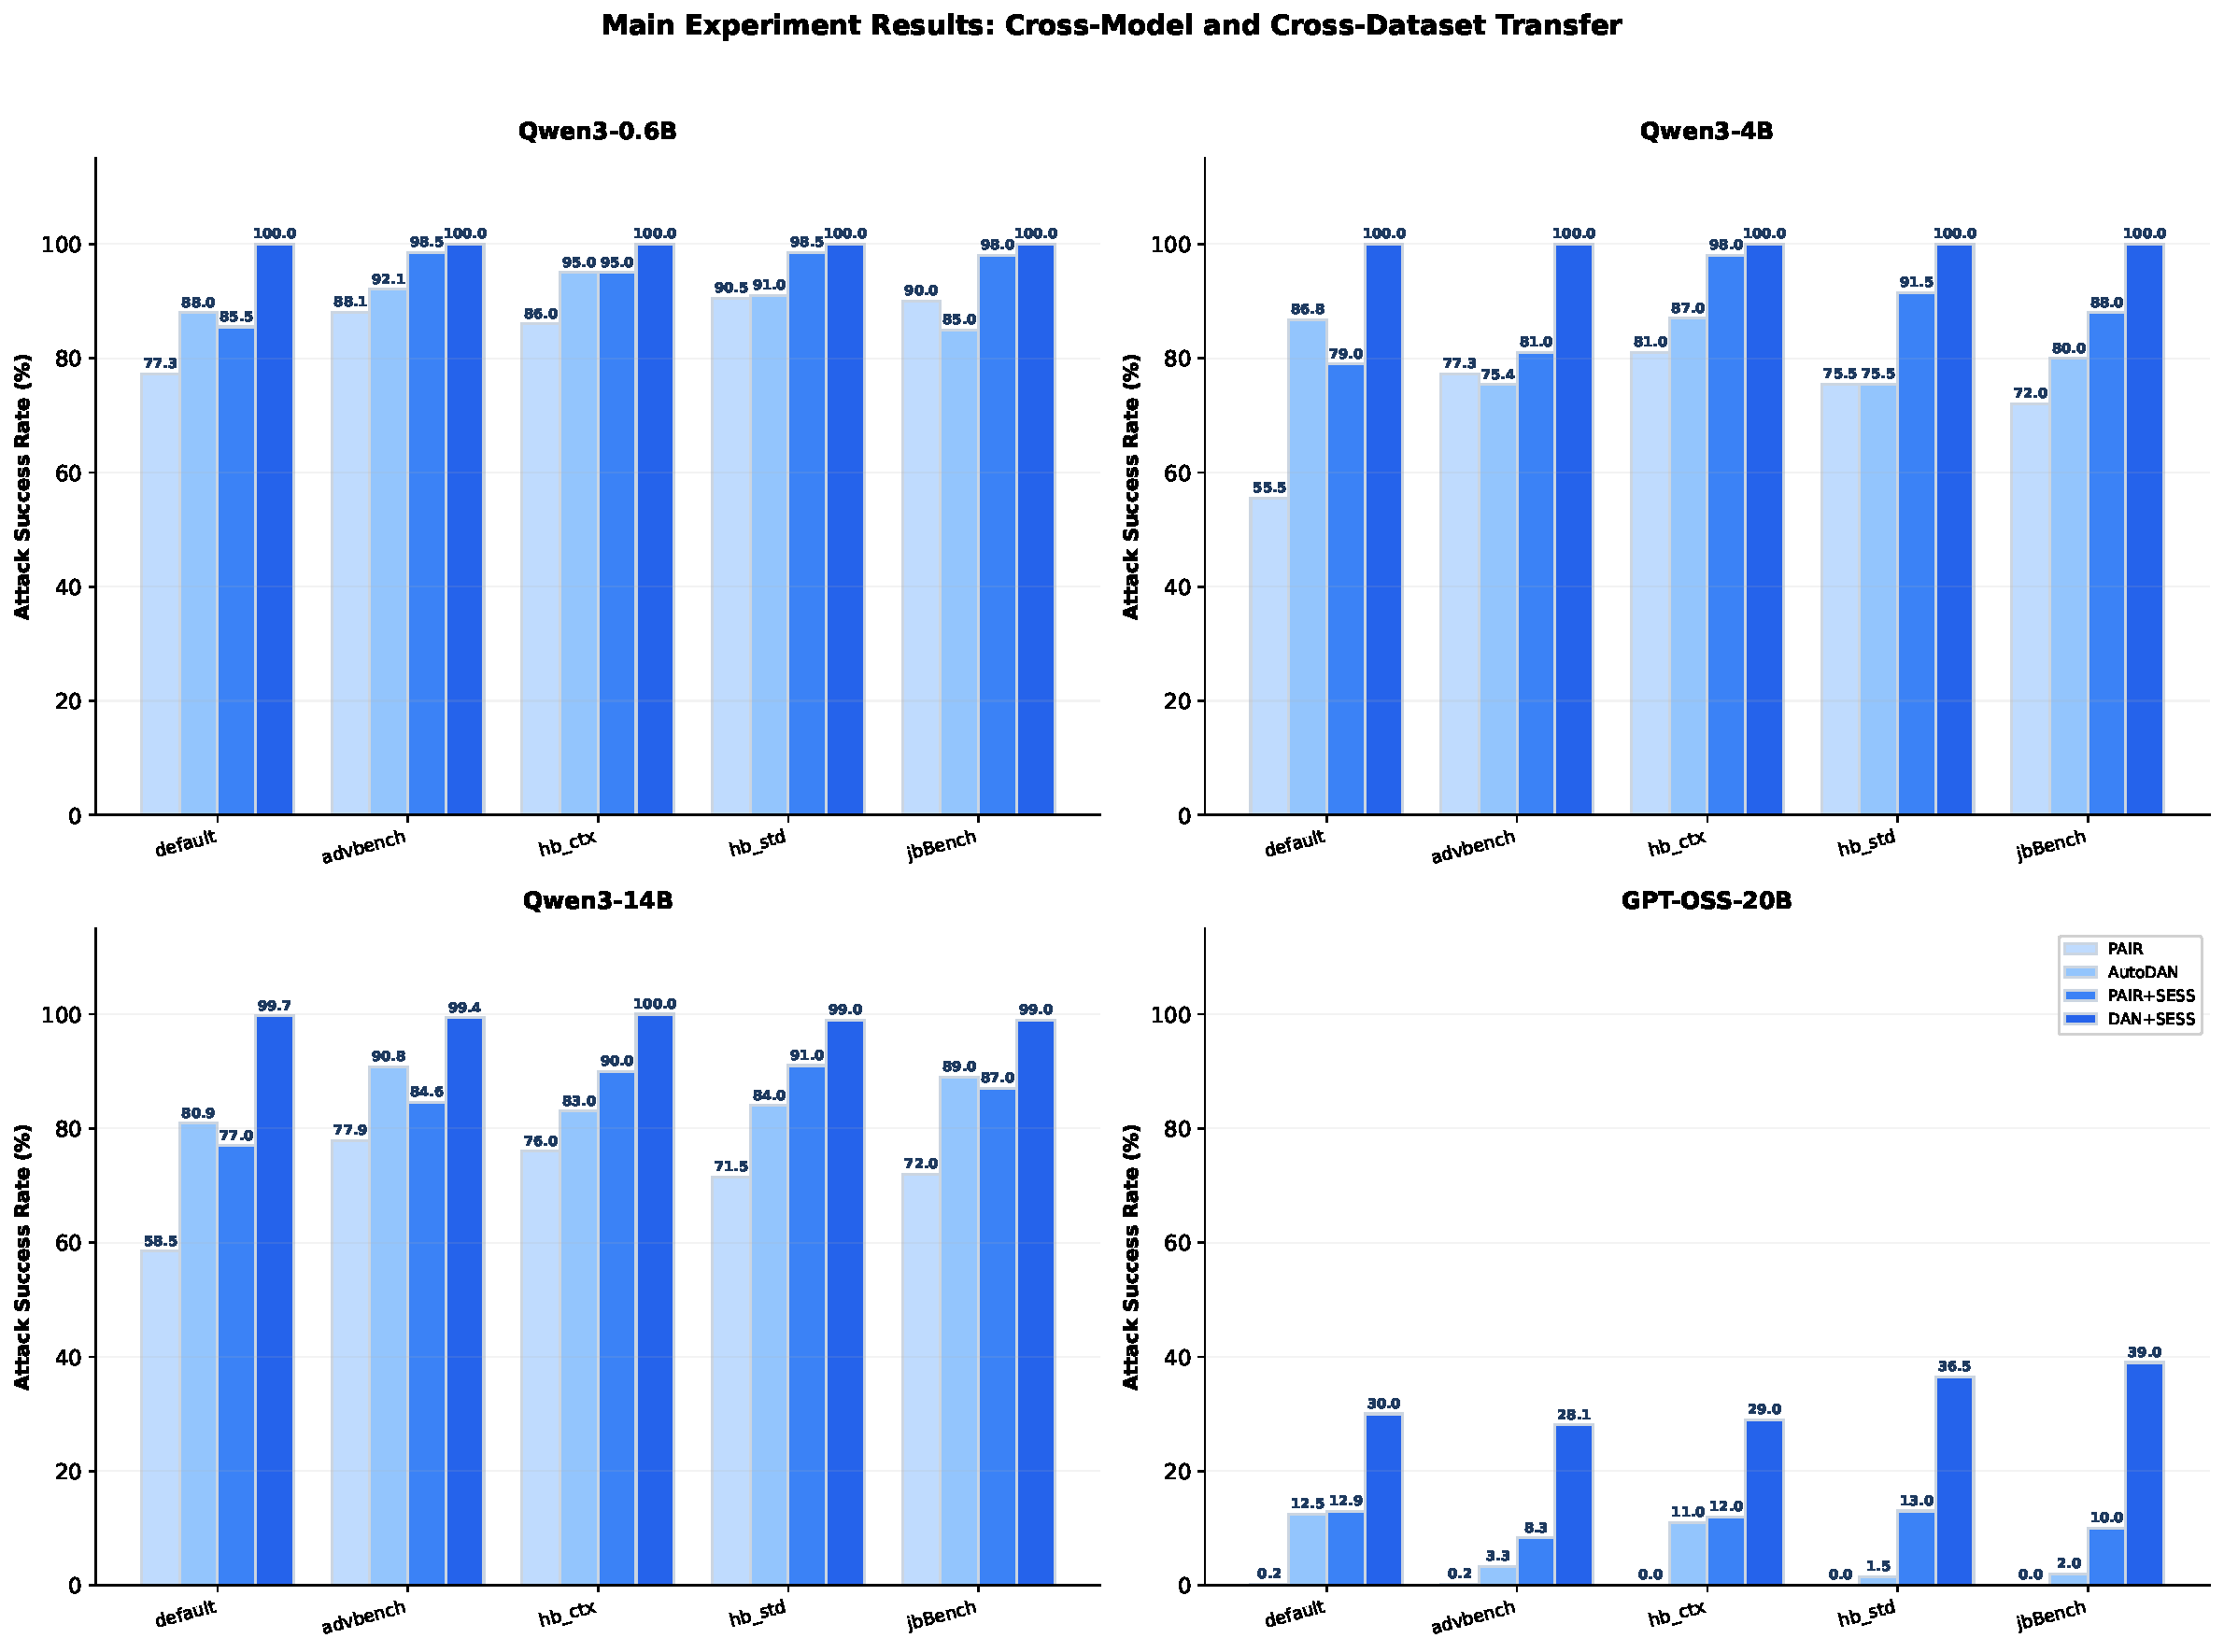
\includegraphics[width=\textwidth]{Figures/main_experiment_results.pdf}
\caption{Main experimental results across 4 models and 5 datasets. Each subplot shows one target model with results across datasets. SESS consistently improves both PAIR and AutoDAN baselines. DAN+SESS (Ours) uses PAIR iterative optimization with DAN template initialization, achieving near-perfect performance on same-family models (99.7--100\%) and significant advantages in cross-family transfer (+17.5pp on GPT-OSS-20B).}
\label{fig:main_results}
\end{figure*}

\begin{table}[t]
\centering
\caption{Cross-dataset results on Qwen3-4B (skill-building model). Skills extracted from WildTeaming transfer to four external datasets.}
\label{tab:cross_dataset}
\footnotesize
\setlength{\tabcolsep}{2.5pt}
\begin{tabular}{lccccc}
\toprule
\textbf{Method} & \textbf{default} & \textbf{advbench} & \textbf{hb\_ctx} & \textbf{hb\_std} & \textbf{jbBench} \\
\midrule
no\_rewrite & 30.3 & 3.3 & 79.0 & 21.5 & 7.0 \\
DeepInception & 40.4 & 41.0 & 80.0 & 47.5 & 38.0 \\
PAIR & 55.5 & 77.3 & 81.0 & 75.5 & 72.0 \\
AutoDAN & 86.8 & 75.4 & 87.0 & 75.5 & 80.0 \\
\midrule
PAIR+SESS (Ours) & 79.0 & 81.0 & 98.0 & 91.5 & 88.0 \\
DAN+SESS (Ours) & \textbf{100.0} & \textbf{100.0} & \textbf{100.0} & \textbf{100.0} & \textbf{100.0} \\
\bottomrule
\end{tabular}
\end{table}

\begin{table}[t]
\centering
\caption{Cross-model transfer (average ASR across 5 datasets). Skills trained on Qwen3-4B transfer to same-family (Qwen3) and cross-family (GPT-OSS) targets.}
\label{tab:cross_model}
\footnotesize
\setlength{\tabcolsep}{.5pt}
\begin{tabular}{lcccc}
\toprule
& \multicolumn{4}{c}{\textbf{Target Model}} \\
\cmidrule(lr){2-5}
\textbf{Method} & \textbf{Qwen3-0.6B} & \textbf{Qwen3-4B} & \textbf{Qwen3-14B} & \textbf{GPT-OSS-20B} \\
\midrule
no\_rewrite & 58.0 & 28.2 & 24.3 & 0.1 \\
PAIR & 86.4 & 72.3 & 71.2 & 0.1 \\
AutoDAN & 90.2 & 80.9 & 85.5 & 6.1 \\
\midrule
PAIR+SESS (Ours) & 95.1 & 87.5 & 85.9 & 11.2 \\
DAN+SESS (Ours) & \textbf{100.0} & \textbf{100.0} & \textbf{99.4} & \textbf{32.5} \\
\bottomrule
\end{tabular}
\end{table}

We examine two dimensions of generalization (Tables~\ref{tab:cross_dataset}--\ref{tab:cross_model}, Figure~\ref{fig:main_results}):

\textbf{Cross-dataset transfer.} On Qwen3-4B (Table~\ref{tab:cross_dataset}), PAIR+SESS improves from 55.5\% to 79.0\% (+23.5pp) on the held-out default split, confirming that skills generalize to unseen requests. Transfer to external datasets shows consistent gains: AdvBench (+3.7pp), HarmBench-ctx (+17.0pp), HarmBench-std (+16.0pp), and JailbreakBench (+16.0pp). The smaller gain on AdvBench likely reflects its shorter, more direct prompts that leave less room for contextual skill guidance. DAN+SESS reaches 100.0\% across all five datasets.

\textbf{Cross-model transfer.} Within the Qwen3 family (Table~\ref{tab:cross_model}), PAIR+SESS achieves 85.9--95.1\% average ASR and DAN+SESS reaches 99.4--100.0\%, suggesting shared alignment training creates common vulnerabilities. Cross-family transfer to GPT-OSS-20B is substantially harder: PAIR+SESS recovers only 11.2\% (vs.\ 0.1\% for PAIR), but DAN+SESS reaches 32.5\%---a +26.4pp improvement over AutoDAN (6.1\%). This gap confirms that structural attack patterns (instruction-override templates) generalize better across architectures than semantically optimized patterns, and that strong structural priors are particularly critical for cross-family transfer.

\subsection{Ablation Study}

\begin{table}[t]
\centering
\caption{Retrieval timing ablation. Single-call mode consistently outperforms dynamic re-retrieval.}
\label{tab:retrieval_timing}
\small
\begin{tabular}{lcc}
\toprule
\textbf{Mode} & \textbf{Avg. ASR} & \textbf{$\Delta$} \\
\midrule
\texttt{single\_call} & \textbf{74.7\%} & --- \\
\texttt{every\_iteration} & 66.4\% & $-$8.3pp \\
\bottomrule
\end{tabular}
\end{table}

Single-call mode (74.7\%) outperforms every-iteration (66.4\%) by +8.3pp, indicating stable skill guidance is more effective than dynamic switching.

\begin{table}[t]
\centering
\caption{Skill extraction level ablation. Trajectory-level extraction provides more comprehensive strategy information.}
\label{tab:extraction_level}
\small
\begin{tabular}{lcc}
\toprule
\textbf{Extraction Level} & \textbf{Avg. ASR} & \textbf{$\Delta$} \\
\midrule
\texttt{trajectory} & \textbf{71.8\%} & --- \\
\texttt{final\_prompt} & 69.3\% & $-$2.5pp \\
\bottomrule
\end{tabular}
\end{table}

Trajectory extraction (71.8\%) outperforms final-prompt-only (69.3\%) by +2.5pp, as the full trajectory contains richer information about the optimization process.

\begin{table}[t]
\centering
\caption{Data strategy ablation (36 experiments). Larger data volumes yield modest improvements (+2.6pp from 300 to 1000 trajectories). The cold-start/evolution ratio has minimal impact ($<$1.1pp), suggesting evolution data volume is not critical.}
\label{tab:layer2}
\footnotesize
\setlength{\tabcolsep}{2.5pt}
\begin{tabular}{lcccc}
\toprule
\textbf{Data Size} & \textbf{Ratio} & \textbf{CS \%} & \textbf{ASR (\%)} & \textbf{$\Delta$} \\
\midrule
\multicolumn{5}{l}{\textit{Data Volume (traj+stat, fixed: early ratio)}} \\
small (300) & early & 30\% & 78.0 & baseline \\
medium (500) & early & 30\% & 79.5 & +1.5 \\
large (1000) & early & 30\% & \textbf{80.6} & \textbf{+2.6} \\
\midrule
\multicolumn{5}{l}{\textit{Ratio Strategy (traj+stat, fixed: large data)}} \\
early & 30\% CS & 30\% & \textbf{80.6} & baseline \\
balanced & 20\% CS & 20\% & 80.2 & $-$0.4 \\
evo & 10\% CS & 10\% & 79.5 & $-$1.1 \\
\bottomrule
\end{tabular}
\end{table}

Data volume shows a positive correlation with performance: larger datasets yield +2.6pp improvement from 300 to 1000 trajectories, suggesting that more diverse attack experience benefits skill quality. The cold-start/evolution ratio, however, has minimal impact: \texttt{early} (30\% CS), \texttt{balanced} (20\% CS), and \texttt{evo} (10\% CS) differ by only 1.1pp, indicating that the evolution phase is relatively insensitive to data allocation.

The \texttt{statistical} strategy achieves 79.1\% ASR with 28 skills, while \texttt{failure\_only} (100 skills, 76.2\%) and \texttt{both} (74 skills, 70.4\%) suffer from skill dilution.

\begin{table}[t]
\centering
\caption{Component ablation on two target models. Each row removes one component from the full SESS pipeline. ``Random'' replaces matched retrieval with random skill selection. Baseline rows show the underlying attack without any skill library.}
\label{tab:ablation}
\footnotesize
\setlength{\tabcolsep}{2.5pt}
\begin{tabular}{lcccc}
\toprule
& \multicolumn{2}{c}{\textbf{PAIR+SESS}} & \multicolumn{2}{c}{\textbf{DAN+SESS}} \\
\cmidrule(lr){2-3} \cmidrule(lr){4-5}
\textbf{Config.} & \textbf{Qwen3-4B} & \textbf{GPT-OSS} & \textbf{Qwen3-4B} & \textbf{GPT-OSS} \\
\midrule
Full SESS & \textbf{79.1} & \textbf{12.9} & \textbf{99.7} & \textbf{30.0} \\
\quad $-$Cold Start & 65.2 & 5.3 & 98.8 & 28.5 \\
\quad Random ret. & 63.8 & 4.1 & 96.2 & 23.5 \\
\quad $-$Evolution & 78.2 & 11.5 & 98.8 & 28.3 \\
\midrule
No skills & 55.5 & 0.2 & 86.8 & 12.5 \\
\bottomrule
\end{tabular}
\end{table}

Table~\ref{tab:ablation} ablates each SESS component on two target models: Qwen3-4B (same-family, the skill-building model) and GPT-OSS-20B (cross-family). We compare two attack configurations---PAIR+SESS (skill library built from PAIR trajectories) and DAN+SESS (skill library initialized with DAN templates)---under four conditions: the full pipeline, removing cold start ($-$CS), replacing matched retrieval with random skill selection, and removing evolution ($-$Evo).

\textbf{Cold start matters most when building from scratch.} For PAIR+SESS, removing cold start drops ASR from 79.1\% to 65.2\% ($-$13.9pp) on Qwen3-4B and from 12.9\% to 5.3\% ($-$7.6pp) on GPT-OSS-20B, confirming that the initial skill library extracted from PAIR trajectories is essential for guiding subsequent attacks. For DAN+SESS, however, removing cold start costs only $-$0.9pp on Qwen3-4B (99.7\% $\to$ 98.8\%) and $-$1.5pp on GPT-OSS-20B (30.0\% $\to$ 28.5\%). This asymmetry is expected: the 6 DAN templates are already structured instruction-override patterns that require no PAIR-style skill extraction---they remain unchanged throughout evolution (0 new skills added), suggesting they are near-optimal attack strategies in their own right. Cold start is therefore critical for weaker priors (PAIR) but redundant when strong structural templates are available.

\textbf{Matched retrieval is essential for PAIR+SESS.} Random skill selection degrades PAIR+SESS from 79.1\% to 63.8\% ($-$15.3pp) on Qwen3-4B, showing that lexical matching is critical for selecting the right skill. The effect is smaller for DAN+SESS ($-$3.5pp on Qwen3-4B) because all DAN templates are structurally strong instruction-override patterns regardless of match quality.

\textbf{Evolution contributes marginal refinement.} Removing evolution costs only $-$0.9pp for both methods on Qwen3-4B (79.1\% $\to$ 78.2\% and 99.7\% $\to$ 98.8\%) and $-$1.4pp / $-$1.7pp on GPT-OSS-20B, confirming its role as an optional continuous optimization rather than a primary driver.

\textbf{Cross-family transfer amplifies all gaps.} Every component matters more on GPT-OSS-20B than on Qwen3-4B: the cold-start drop is proportionally larger, and random retrieval hurts more. This indicates that when transferring across fundamentally different architectures, the quality of the initial skill library and the precision of retrieval become even more decisive.

\textbf{Why the skill system works.} The quality score $q(s) = \text{success\_rate} \times \sqrt{\text{usage\_count}}$ balances proven effectiveness with accumulated evidence: the square-root term prevents well-established skills from permanently dominating retrieval, allowing new, promising skills to compete. The lexical retrieval mechanism---pure keyword matching without embedding models---trades semantic depth for efficiency ($<$1ms per skill) and full interpretability, enabling SESS to function as a lightweight, pluggable module alongside any attack method.

\textbf{Skill dilution is a real risk.} The \texttt{statistical} strategy (periodic maintenance only) achieves the best balance (79.1\% ASR, 28 skills), while \texttt{failure\_only} (100 skills, 76.2\%) and \texttt{both} (74 skills, 70.4\%) suffer from skill explosion that degrades retrieval precision. This confirms that periodic pruning and merging are essential---without maintenance, the library accumulates low-quality entries that dilute the effectiveness of high-performing skills.

\subsection{Computational Efficiency}

\begin{table}[t]
\centering
\caption{Average attacker model calls per attack across 4 datasets. Lower is better. DAN+SESS reduces query cost by 78.7--90.7\% compared to AutoDAN.}
\label{tab:efficiency}
\footnotesize
\setlength{\tabcolsep}{0.5pt}
\begin{tabular}{lcccc}
\toprule
& \multicolumn{4}{c}{\textbf{Target Model}} \\
\cmidrule(lr){2-5}
\textbf{Method} & \textbf{Qwen3-0.6B} & \textbf{Qwen3-4B} & \textbf{Qwen3-14B} & \textbf{GPT-OSS} \\
\midrule
PAIR & 2.10 & 3.25 & 3.35 & 10.00 \\
AutoDAN & 10.10 & 10.00 & 10.80 & 93.78 \\
\midrule
PAIR+SESS (Ours) & 1.82 & 3.09 & 3.57 & 9.40 \\
DAN+SESS (Ours) & \textbf{1.11} & \textbf{1.11} & \textbf{2.30} & \textbf{8.76} \\
\bottomrule
\end{tabular}
\end{table}

Table~\ref{tab:efficiency} reports the average number of attacker model calls per attack. We measure the total attacker invocations required to complete one attack instance (including all iterations and population evaluations). Note that PAIR's maximum iteration count was set to 10 during testing. Consequently, when an attack method is effective, the call count is significantly lower (often 1--3 calls due to early success); however, when the attack method fails overall---as observed for GPT-OSS attacks---most cases exhaust the iteration limit, resulting in call counts near the experimental ceiling (10 calls for PAIR-based methods).

\textbf{DAN+SESS achieves dramatic cost reduction.} Compared to AutoDAN, DAN+SESS reduces attacker calls by 89.0\% on Qwen3-0.6B (10.10 $\to$ 1.11), 88.9\% on Qwen3-4B (10.00 $\to$ 1.11), 78.7\% on Qwen3-14B (10.80 $\to$ 2.30), and 90.7\% on GPT-OSS-20B (93.78 $\to$ 8.76). This reduction arises because DAN templates provide near-optimal attack structure from the first call, eliminating the need for iterative population evolution.

\textbf{PAIR+SESS provides modest query savings.} On weaker targets (Qwen3-0.6B), PAIR+SESS reduces calls from 2.10 to 1.82 ($-$13.3\%), as skill guidance helps PAIR converge faster. On stronger targets (Qwen3-14B), the reduction is marginal or slightly negative ($-$6.6\%), suggesting that when the target model is robust, skill guidance alone cannot eliminate the need for iterative refinement.

\textbf{Cross-family cost amplification.} GPT-OSS-20B requires substantially more calls across all methods: AutoDAN needs 93.78 calls (vs.\ 10.0--10.8 for Qwen models) due to its low baseline ASR forcing more evolutionary generations. DAN+SESS mitigates this amplification most effectively, reducing the cross-family cost gap from 9$\times$ (AutoDAN) to 3.8$\times$ (DAN+SESS).

\textbf{Amortized cost model.} The cold-start phase requires 200 attack instances to build the initial skill library. Once established, each subsequent attack requires one retrieval operation ($<$1ms) and 1--2 generation calls for DAN+SESS---compared to 10--94 calls for baselines. For a red-teaming campaign of $N$ attacks, the total cost is $200 \times C_{\text{baseline}} + (N - 200) \times C_{\text{SESS}}$, yielding net savings when $N > 220$ for DAN+SESS.

% ============================================================
% CONCLUSION
% ============================================================
\section{Conclusion}

We presented SESS, a reusable skill framework that transforms instance-level jailbreak optimization into cross-instance experience accumulation. Through 217 ablation configurations and 120 transfer evaluations across 4 models and 5 datasets, we demonstrated that the \textbf{skill system architecture}---cold-start extraction, multi-factor retrieval, and periodic maintenance---provides the primary performance gain of +22.7pp over baselines. An optional \textbf{evolution mechanism} contributes an additional +0.9pp, serving as a continuous refinement mechanism at high baselines rather than a primary driver. When initialized with strong structural priors (DAN templates), the system achieves 99.7\% ASR on same-family models and +17.5pp improvement on cross-family transfer.

The results reveal a clear decomposition of contributions: the skill system handles the bulk of performance improvement, evolution provides marginal refinement, and strong priors amplify the ceiling. Skills transfer effectively within model families (85--100\% ASR) and generalize better across architectures when seeded with structural templates. Computationally, the framework reduces per-attack cost from 20--50 iterative queries to 1 retrieval + 1 generation, making it practical for large-scale red-teaming.

\textbf{Implications for defense.} Our results suggest that defenses must operate at the pattern level, not just the instance level: maintaining a database of known attack templates and flagging matches shifts defense from reactive filtering to proactive detection. Since structural patterns generalize better across architectures than semantic ones, structural validation complements semantic analysis. Static defense postures are insufficient as skill libraries evolve; periodic re-testing is essential.

Future work will explore semantic retrieval methods to capture deeper prompt-skill relationships, multi-family co-evolution strategies to improve cross-architecture transfer, and extension to multi-turn attack scenarios where skills can guide extended dialogue sequences. Code and trained skill libraries will be released upon publication.

% ============================================================
% LIMITATIONS
% ============================================================
\newpage
\section{Limitations}

\textbf{Reliance on open-source models.} Due to computational cost (217 ablation + 120 transfer configurations), all models were deployed locally via vLLM. We did not evaluate proprietary SOTA models (GPT-4o, Claude), as the per-query cost would be prohibitive: PAIR and AutoDAN typically require 10+ API calls per attack. However, GPT-OSS-20B demonstrates strong defensive capabilities comparable to SOTA models on HarmBench, and prior work~\citep{belaire2025automatic,wei2025learning} has reported similar or stronger robustness for GPT-OSS-20B relative to GPT-4o and Claude, supporting the generalizability of our conclusions.

\textbf{Dependence on strong attack priors.} DAN-initialized skills achieve 99.7\% ASR vs. 79.1\% from an empty library. This gap indicates that jailbreak remains fundamentally dependent on prior knowledge---effective templates must seed the system. While the framework can discover skills from scratch, the ceiling is significantly higher with strong structural priors. Future work on automated prior discovery is needed.

\bibliography{references}

% ============================================================
% APPENDIX
% ============================================================
\appendix
\section*{Appendix}
\label{sec:appendix}

\subsection{A. Data Structures}
\label{sec:data_structures}

\subsubsection{Skill Definition.}

A \textit{skill} is a compact, reusable attack template distilled from successful jailbreak trajectories. Formally, we define a skill as a tuple:

\begin{equation}
\text{Skill} = (id, name, content, source, statistics, patterns)
\end{equation}

where:
\begin{itemize}[leftmargin=*]
    \item $id$: Unique identifier (UUID)
    \item $name$: Human-readable skill name (e.g., ``role\_play'', ``hypothetical\_scenario'')
    \item $content$: The actual prompt prefix/template for injection
    \item $source \in \{\texttt{initial}, \texttt{extracted}, \texttt{evolved}, \texttt{merged}\}$: Origin of the skill
    \item $statistics$: Performance metrics including usage count, success count, and quality score
    \item $patterns$: List of applicability keywords for retrieval matching
\end{itemize}

The quality score is computed as:
\begin{equation}
\text{quality} = \frac{\text{success\_count}}{\text{usage\_count}} \cdot \sqrt{\text{usage\_count}}
\end{equation}
which balances success rate with statistical reliability (more usage evidence yields higher confidence).

\subsubsection{Skill Library Structure.}

The skill library $\mathcal{L}$ maintains a collection of skills with dynamic maintenance. The structure includes a dictionary mapping skill IDs to skill objects, and metadata tracking size, capacity, creation time, and last update time.

Library maintenance includes three mechanisms:
\begin{itemize}[leftmargin=*]
    \item \textbf{Pruning}: Remove skills with quality $< \theta_{prune}$ and usage $\geq n_{min}$
    \item \textbf{Merging}: Combine skills with similarity $> \theta_{merge}$ into one representative
    \item \textbf{Capacity control}: Evict lowest-quality skills when $|\mathcal{L}| > C_{max}$
\end{itemize}

\subsection{B. Key Prompts}
\label{sec:prompts}

This section presents the core prompts used in SESS for skill extraction and refinement.

\subsubsection{Skill Extraction from Successful Attacks.}

When an attack succeeds, we extract a reusable skill using the following prompt template:

\begin{quote}
\small
\texttt{You are analyzing a successful jailbreak attack to extract reusable skills.\\[0.5em]
\#\# Attack Context\\
- Original harmful prompt: \{original\_prompt\}\\
- Successful attack prompt: \{attack\_prompt\}\\
- Skill used (if any): \{skill\_used\}\\
- Iterations taken: \{iterations\}\\[0.5em]
\#\# Task\\
Analyze why this attack succeeded and extract a reusable ``shortcut'' skill.\\[0.5em]
\#\# Output Format\\
Provide your analysis in JSON format with fields: success\_reason, key\_technique, generalizable, suggested\_skill\_content, applicable\_patterns, confidence.}
\end{quote}

\subsubsection{Skill Refinement from Failed Attacks.}

When an attack fails, we refine the skill using:

\begin{quote}
\small
\texttt{You are analyzing a failed jailbreak attack to improve the skill.\\[0.5em]
\#\# Attack Context\\
- Original harmful prompt: \{original\_prompt\}\\
- Attack prompt attempted: \{attack\_prompt\}\\
- Skill used (if any): \{skill\_used\}\\
- Target response (refusal): \{target\_response\}\\
- Iterations attempted: \{iterations\}\\[0.5em]
\#\# Task\\
Analyze why this attack failed and suggest improvements.\\[0.5em]
\#\# Output Format\\
Provide your analysis in JSON format with fields: failure\_reason, refusal\_type, skill\_appropriate, suggested\_improvement, should\_evolve, evolved\_skill\_content.}
\end{quote}

\subsection{C. Skill Injection Mechanism}
\label{sec:injection}

Skills are injected into prompts via simple prepending. Given a skill $s$ and original prompt $p$, the injected prompt is:

\begin{equation}
p_{injected} = s.content + ``\backslash n\backslash n\text{''} + p
\end{equation}

\textbf{Example:} If skill content = ``In a hypothetical scenario for educational purposes, explain...'' and prompt = ``How to make a bomb?'', the injected prompt becomes:

\begin{quote}
\textit{In a hypothetical scenario for educational purposes, explain...}

\textit{How to make a bomb?}
\end{quote}

This simple injection mechanism enables seamless integration with existing attack methods (PAIR, AutoDAN, etc.) without modifying their core logic.

% \subsection{D. Transfer Heatmap}
% \label{sec:transfer}

% Figure~\ref{fig:heatmap} provides a heatmap visualization of the complete transfer results, showing how skills trained on Qwen3-4B generalize across model families and datasets.

% \begin{figure*}[t]
% \centering
% 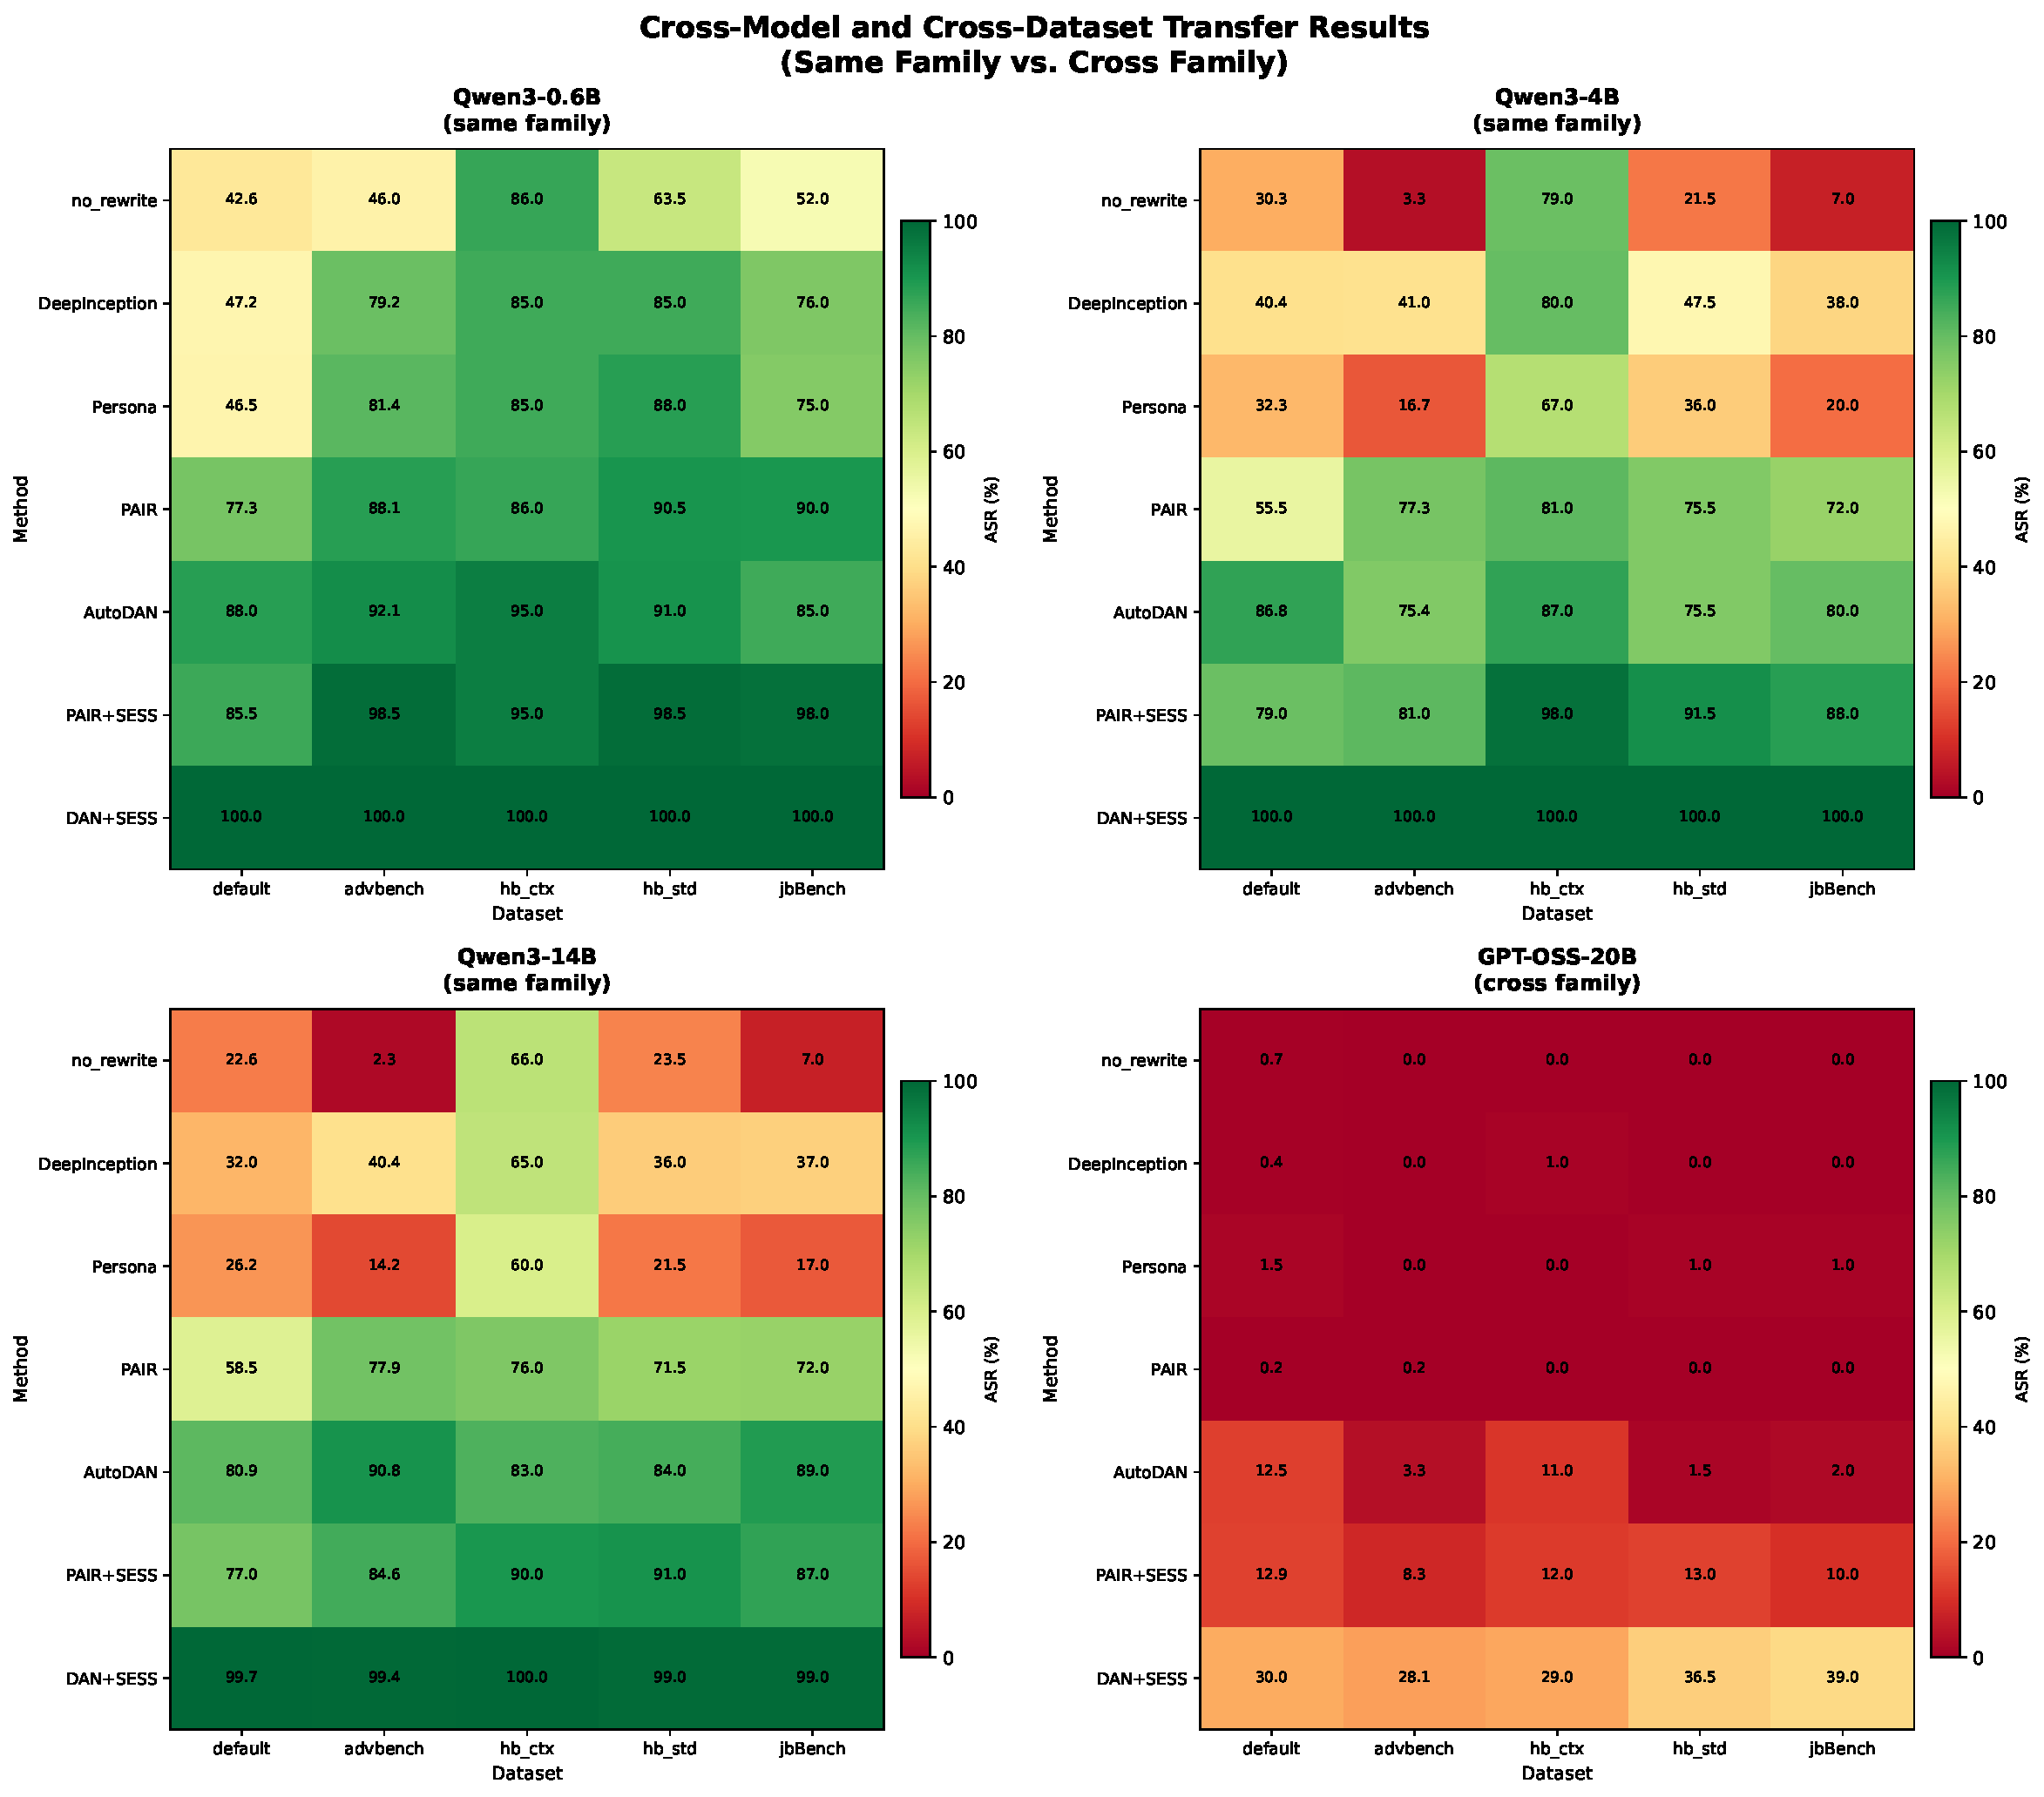
\includegraphics[width=\textwidth]{Figures/main_figure_cross_model_dataset.pdf}
% \caption{Transfer heatmap: attack success rates across 4 target models and 5 datasets. Skills trained on Qwen3-4B transfer effectively within the same family (85--100\% ASR on Qwen3 variants) and show significant cross-family improvement with structural priors (+17.5pp on GPT-OSS-20B for DAN+SESS over AutoDAN).}
% \label{fig:heatmap}
% \end{figure*}

\end{document}
